\documentclass[conference]{IEEEtran}
\IEEEoverridecommandlockouts
% The preceding line is only needed to identify funding in the first footnote. If that is unneeded, please comment it out.
\usepackage{cite}
\usepackage{amsmath,amssymb,amsfonts}
\usepackage{algorithmic}
\usepackage{graphicx}
\usepackage{textcomp}
\usepackage{xcolor}
\def\BibTeX{{\rm B\kern-.05em{\sc i\kern-.025em b}\kern-.08em
    T\kern-.1667em\lower.7ex\hbox{E}\kern-.125emX}}
\begin{document}

\title{Course Project Final Report\\

}

\author{\IEEEauthorblockN{Clayton Tucker}
\IEEEauthorblockA{\textit{COSC325} \\
\textit{Ctrl Alt Delete}\\
Knoxville, US \\
ctucke24@vols.utk.edu}
\and
\IEEEauthorblockN{Todd Van Meter}
\IEEEauthorblockA{\textit{COSC 325} \\
\textit{Ctrl Alt Delete}\\
Knoxville, US \\
tvanmete@vols.utk.edu}
\and
\IEEEauthorblockN{Danyil Chuprynov}
\IEEEauthorblockA{\textit{COSC 325} \\
\textit{Ctrl Alt Delete}\\
Knoxvile, US \\
dchupryn@vols.utk.edu}
\and
\IEEEauthorblockN{Ian Henson}
\IEEEauthorblockA{\textit{COSC 325} \\
\textit{Ctrl Alt Delete}\\
Knoxvile, US \\
tkd995@vols.utk.edu}
}

\maketitle

\begin{abstract}
The stock market is very popular investment as one can earn a significant amount of money, but the major problem is that no one knows how to accurately predict if a stock would go up or down. The purpose of this article is to find a way to accurately predict future stock prices. This can be done by developing a machine learning program that trains itself on previous stock prices. There exist many different learning models to predict the future of stocks, though many of them are not considered efficient enough.The aim of this project is to take an existing learning model and further improve it using learning techniques such as ARIMA, Linear Regression, or Random forests. For this article, we will be using an ARIMA with Long Short Term Based Memory.  We hope to improve it by shortening the data cut-off or perhaps combining multiple learning models.
\end{abstract}

\begin{IEEEkeywords}
Machine Learning, ARIMA, Linear Regression, Random forest, Stock Price Prediction, Moving Average
\end{IEEEkeywords}

\section{Introduction}
Predicting stock prices is a challenging yet critical task in finance due to market volatility and unpredictability. Machine learning provides powerful tools capable of identifying complex patterns within historical financial data, which can lead to more accurate stock price forecasts.

We aim to specifically examine the application of machine learning techniques to predict the stock prices of Berkshire Hathaway, a leading investment firm known for its diverse portfolio and market influence [1]. Accurate prediction models for Berkshire Hathaway's stock could significantly assist investors in making informed decisions, managing investment risks, and capitalizing on market trends.

Utilizing the Berksire-Hathaway historical stock data from Kaggle, we aim to:
\begin{itemize}
    \item Analyze and pre-process historical data to identify predictive features.
    \item Implement and evaluate multiple ML models to determine their forecasting accuracy.
    \item Assess the practical effectiveness of ML in predicting Berkshire Hathaway’s stock performance.
\end{itemize}

Through these objectives, the project seeks to contribute to improving investment strategies and demonstrating the value of ML applications in financial market analysis.

\section{Data Exploration}

\subsection{The Dataset}

The dataset used in this study is the Berkshire Hathaway Stock Price Data, sourced from Kaggle [1]. This dataset includes historical stock information consisting of 1,671 daily samples collected from January 2, 2020, to July 29, 2024. Each sample contains eight features: open price, high price, low price, close price, adjusted close price, trading volume, log-transformed closing price, and date converted to an ordinal number format. The dataset is continuous and inherently balanced as it involves time-series data rather than categorical classes. The dataset also contains major events, such as the COVID-19 Pandemic, which heavily skewed it.Due to its nature, it requires special pre-processing techniques, such as stationary adjustments and log transformations, to ensure effective application of predictive models.

\subsection{Preprocessing}
Detailed preprocessing steps applied to the data included:
\begin{itemize}
    \item Filtering to include only data from January 2020 onwards to maintain consistency and relevance.
    \item Handling missing values by forward-filling daily gaps to maintain continuity, ensuring no temporal discontinuities in the dataset.
    \item Transforming the 'Close' price feature using a logarithmic scale to stabilize variance and manage heterogeneity of variance.
    \item Calculating the first-order differences on all features to achieve stationarity, a requirement for ARIMA modeling, confirmed through the Augmented Dickey-Fuller (ADF) test.
    \item Then a moving average and standard deviation features was calculated to improve accuracy, the latter was required for ARIMA.
\end{itemize}

The preprocessing steps above were critical to improving and ensuring the effectiveness of the predictive models employed in this study.

\subsection{Data Analysis}\label{AA}
\begin{itemize}
    \item \textbf{Overall Stock Price Trend}: Berkshire Hathaway's stock price exhibited an increasing trend over the analyzed period from January 2020 to July 2024. The closing price started around \$228 in early 2020 and rose significantly, reaching approximately \$438 in July of 2024, suggesting overall growth and positive long-term performance.
    \item \textbf{Seasonality and Stationarity}: Initial tests for stationarity ADF test indicated non-stationarity in raw closing prices (Test Statistic: -0.52, P-Value: 0.89). Thus, data transformations (log differences) were applied to make the dataset stationary, which is essential for effective ARIMA modeling.
    \item \textbf{Volume Insights}: The daily traded volume shows significant variability, indicating periods of increased investor activity. The high volatility in trading volume suggests events or news that significantly influenced investor behavior and stock prices.
     \includegraphics[scale=0.25]{linregdone.png} %screenshots/linreg.png
    \item \textbf{Model Performance Comparison}: ARIMA and Random Forest models produced similar predictive accuracy (RMSE approximately 22.2 and 22.1, respectively), outperforming Linear Regression, which had notably higher errors (RMSE approximately 31.6). This confirms non-linearity in stock price data and highlights the effectiveness of non-linear models like ARIMA and Random Forest.
    \\
     \includegraphics[scale=0.25]{linregdone.png} %screenshots/linreg.png
     \\
      \includegraphics[scale=0.25]{ranfordone.png} %screenshots/ranfor.png
    \\
       \includegraphics[scale=0.25]{arimadonenow.png} %screenshots/arima.png
    \item \textbf{Error Analysis}: Both ARIMA and Random Forest displayed relatively low and similar absolute errors (~18), indicating that while there are predictive limitations, both models adequately captured short-term movements in stock prices.
    \item \textbf{Possible Overfitting with Random Forest}: Random Forest exhibited consistent predictions across test days (constant values), suggesting possible overfitting to the training data. While it resulted in low errors, the model’s predictions lacked variability, potentially limiting its usefulness in dynamic real-world trading scenarios.
\end{itemize}

\section{Baseline Model}

Before we can process our dataset, we must first decide the best possible model as our baseline. As there are many different baselines, all with their strengths and weaknesses, we explored some of the existing solutions to determine which one to use.

\subsection{Existing Solutions}

\begin{itemize}

    \item \textbf{Linear Regression}: Linear Regression is a simple model that people have used for stock market predictions. However, after using a Linear Regression model on our data, our predictions were linear and flat. This is likely due to our data being nonlinear, making Linear Regressions an unideal model to use.   

    \item \textbf{Random Forests}: Another popular model used in stock market predictions is Random Forests. Random Forests, compared to Linear Regression, is capable of handling non-linear data and provides better results such as a lower MSE. There is some drawbacks, as random forests struggles with time series data.

    \item \textbf{ARIMA}: ARIMA models are also well known in stock market predictions and considered one of the best among other models[2]. Just like Random Forests, ARIMA models can handle non-linear data, but requires the data to be stationary for best performance. 

    \item \textbf{Moving Average}: Moving Average is another consideration as they have been widely used before. They are known being able to be tailored to different time-frames and smoothing price-data, but requires extra implementations, such as a Regression model, to fine-tune signal delays[2].

\end{itemize}

\subsection{Baseline Model}

For our baseline model, we chose the ARIMA (AutoRegressive Integrated Moving Average) algorithm due to its well-established capability in modeling and forecasting time series data. ARIMA has been a popular approach in financial modeling for some time, with many prior works using it as a benchmark in predictions [1].
Our implementation followed the approach outlined in a Kaggle notebook titled Stock Prices Prediction Using Classic Auto ARIMA, which provided a solid foundation for our goal of predicting the stock price. We started by transforming our close price by log. This was to stabilize variance and reduce the noise found in the dataset. Next, we tested the data for stationary, which is a requirement for data being used in an ARIMA model, using the Augmented Dickey-Fuller (ADF) test. The results concluded that our dataset was non-stationary, which had us apply differencing techniques to remove trends and seasonality.
Then, to determine our hyperparameter for the model, we manually examined the Auto Correlation Function (ACF) and Partial Auto Correlation Function (PACF) plots. This led us to select p=0, d=1, q=0 for our configuration. After training the model, we evaluated it on our test set (80/20) split and got a Root Mean Square Error (RMSE) of 22.24.
To compare this model, we also trained a classic Linear Regression model and a Random Forest Regressor. These had an RMSE value of 31.58 and 22.09, respectively. Although the random forest performed slightly better than the ARIMA model in terms of error, it lacked the time series awareness that ARIMA provides. Linear regression performed the worst due to its inability to capture non-linear and sequential trends in stock prices.
From our testing, we concluded that each model had its own strengths and weaknesses. ARIMA was able to handle time series data but struggled with capturing non-linear behavior. Our Random Forest performed better when learning non-linear behavior but did not model time dependency well. 
These findings motivated our plan to create an ensemble model between ARIMA and Random Forest, with ARIMA modeling the trend and Random Forest capturing the residual, non-linear variations. Our goal was to combine their strengths and reduce overall error in future iterations.

\section{Model Improvements}



The initial model development utilized basic ARIMA, Linear Regression, and Random Forest models to establish a baseline for predicting stock prices. After analyzing the preliminary results, we implemented the following key improvements:

\begin{enumerate}
    \item ARIMA to SARIMA Transition: After looking at the seasonal decomposition of the time series data, we identified significant seasonal patterns that the classic ARIMA model failed to capture. By implementing SARIMA (seasonal ARIMA), we enhanced the model’s ability to account for these patterns. We aimed to reduce the impact seasonality would have within our dataset, but SARIMA was able to strength our model further.
    
    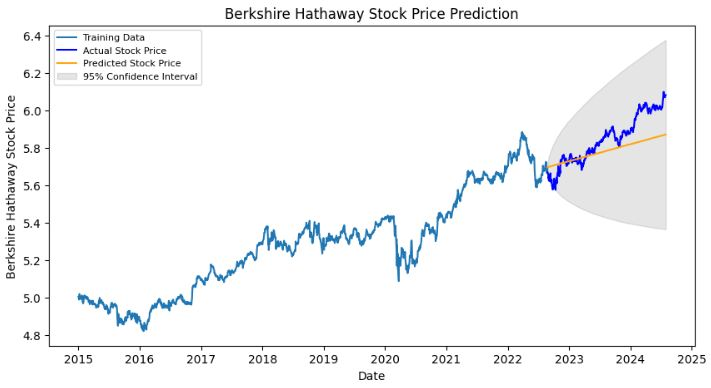
\includegraphics[scale=0.50]{SARIMA_results.JPG} %final-screenshots/SARIMA_results.jpg

    \item Auto-ARIMA Parameter Optimization: Rather than relying on manual calculations to optimize our hyper parameters, we implemented Auto-ARIMA to calculate the most optimal configuration. This process determined that (2,1,0) was the strongest combination.
    
    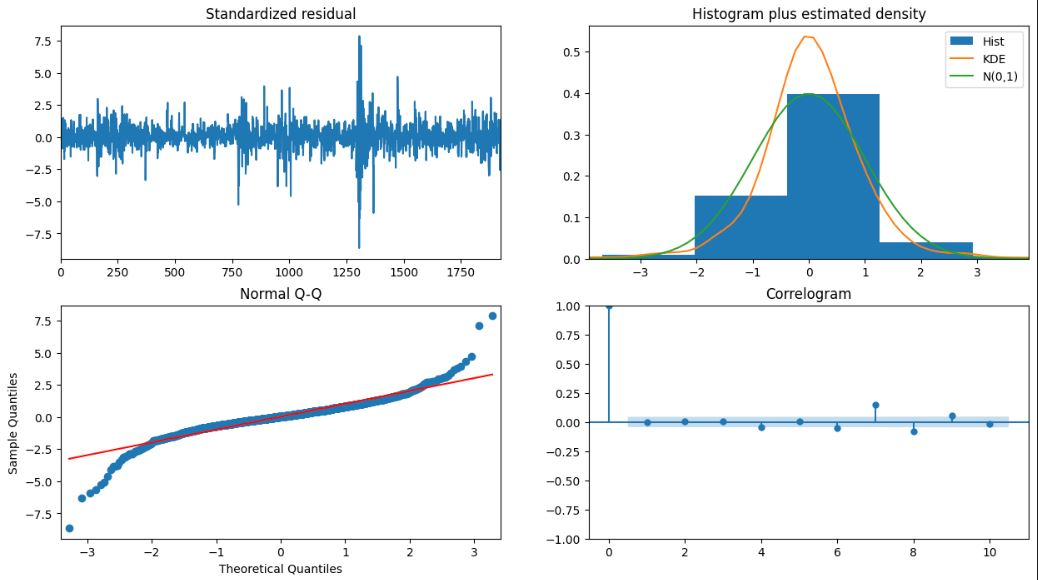
\includegraphics[scale=0.30]{auto_arima_results.JPG} %final-screenshots/auto_arima_results.jpg

    \item Ensemble Approach: To leverage the pros and cons of the SARIMA and Random Forest Regressor models, we implemented a dynamically weighted strategy. Using a rolling window of 10 time steps, we calculated the recent Mean Squared Error (MSE) of each model’s predictions. We then applied inverse-error weighting to the predictions, giving a higher weight to the model with a lower error. At each step, the ensemble prediction was computed as a weighted average of the two models’ output using the weights. This allowed the ensemble to adapt over time, reducing the error and emphasizing the better performing model.
    
    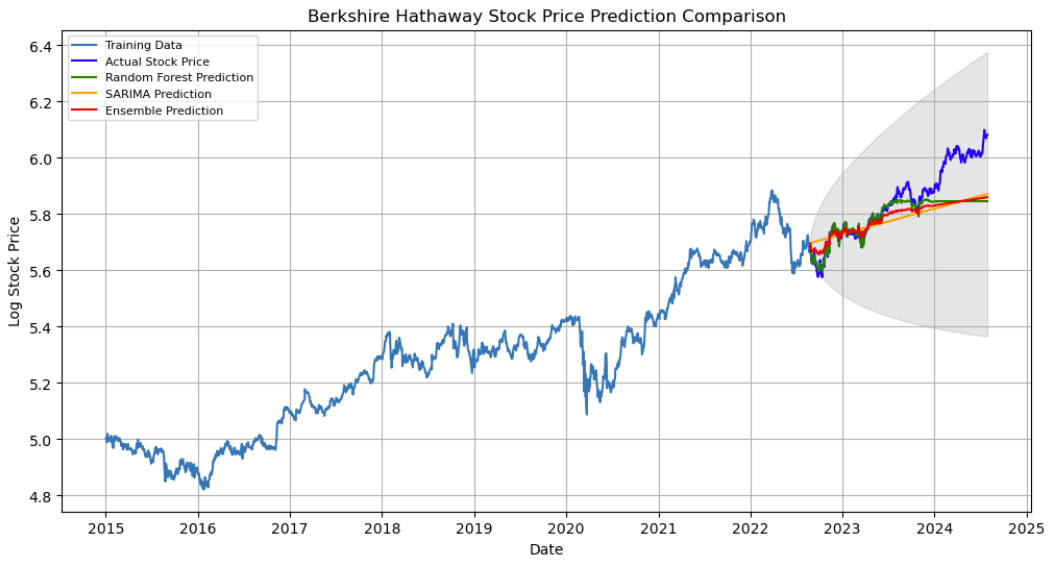
\includegraphics[scale=0.40]{Ensemble_results.png} %final-screenshots/ensemble_results

\end{enumerate}


\textbf{Performance Evaluation:}

\begin{enumerate}

    \item Mean Square Error (MSE):

    \begin{enumerate}
        \item SARIMA: 0.00999
        \item Random Forest: 0.0081
        \item Ensemble: 0.0073
    \end{enumerate}

    \item Mean Absolute Error (MAE):
    
    \begin{enumerate}
        \item SARIMA: 0.0801
        \item Random Forest: 0.0577
        \item Ensemble: 0.061
    \end{enumerate}

    \item Root Mean Squared Error (RMSE):

    \begin{enumerate}
        \item SARIMA: 0.099
        \item Random Forest: 0.090
        \item Ensemble: 0.0859
    \end{enumerate}    

    \item Confidence Intervals: For the model, we calculated 95\% confidence intervals to quantify the prediction uncertainty of our model, visualized by the shaded regions. 

    
\end{enumerate}

\textbf{Model Performance Analysis:}

The Random Forest model performed roughly 10\% better in all of our evaluation metrics. This suggests that the non-linear patterns in the stock prices are significant factors that time series models struggle to capture.
However, when both models are combined with dynamic weights, the benefits of each model help to reduce the overall error. As our Random Forest Regressor started to plateau, the SARIMA model helped pick up the weight. 
The confidence intervals help show the wider uncertainty during periods of higher volatility in the market. One example of this is the COVID-19 market disruption in 2020.

\textbf{Conclusion:}

This study investigated the effectiveness of various modeling approaches for stock price prediction. Combining the strength of two independently strong models used for stock prediction, we were able to improve the accuracy of prediction utilizing dynamic weights. Our findings show several key insights that contribute to the broader understanding of stock prediction methods. 
The baseline ARIMA model provided a solid foundation for time series prediction, demonstrating reasonable performance with a root mean square error of 0.099. However, this traditional approach exposed limitations in capturing more complex patterns within the closing price of a single stock. In contrast, the Random Forest Regressor showed its strengths in modeling non-linear relationships, giving a better RMSE of 0.09. 
During our model refinement process, we uncovered the strength of both of these models. When switching from the classic ARIMA model to a SARIMA model to better capture seasonality, fine tuning our hyperparameters with auto-ARIMA, and most importantly utilizing our approach for a dynamically weighted ensemble approach. We were able to improve our model’s error down to 0.0859, outperforming both models.

\section{Distribution of Work}
All members of the team equally contributed to getting this midterm report finished.  Danyil Chuprynov and Ian Henson both researched implementation of model baselines and worked on developing the code.  Todd Van Meter and Clayton Tucker researched the effectiveness of these models and wrote the majority of the report in the beginning, and in the end we all came together to write the final report.

\begin{thebibliography}{00}
\bibitem{b1} Umer Haddii, “Berkshire Hathaway Stock Price Data,” Kaggle.com, 2024. https://www.kaggle.com/datasets/umerhaddii/berkshire-hathaway-stock-price-data
\bibitem{b2} vafaknm, “stock prices prediction using classic/auto ARIMA,” Kaggle.com, Sep. 11, 2022. https://www.kaggle.com/code/vafaknm/stock-prices-prediction-using-classic-auto-arima\#Berkshire-Hathaway (accessed May 03, 2025).
\end{thebibliography}

\end{document}
